% latex table generated in R 3.6.3 by xtable 1.8-4 package
% Thu Jan 18 11:48:16 2024
\begin{table}[ht]
\centering
\begin{tabular}{rlrrr}
  \hline
 & OTU & MeanRA & MedianRA & SE \\ 
  \hline
634177 & Komagataeibacter medellinensis & 0.00004533 & 0.00004546 & 0.00000264 \\ 
  1840265 & Polaromonas sp. E3 & 0.00000699 & 0.00000611 & 0.00000152 \\ 
  32009 & Burkholderia gladioli & 0.00005177 & 0.00005275 & 0.00000265 \\ 
  521 & Bordetella aviu & 0.00006274 & 0.00007261 & 0.00000990 \\ 
  490 & Neisseria sicc & 0.00001410 & 0.00001254 & 0.00000252 \\ 
  2498848 & Pseudomonas sp. MPC & 0.00005685 & 0.00005099 & 0.00000709 \\ 
  2726956 & Pseudomonas sp. MSPm & 0.00007321 & 0.00005263 & 0.00001755 \\ 
  2320270 & Pseudomonas sp. DG56- & 0.00004746 & 0.00004076 & 0.00000691 \\ 
  2774873 & Pseudomonas sp. ADP & 0.00005470 & 0.00004446 & 0.00000911 \\ 
  658644 & Pseudomonas sp. R5-89-0 & 0.00003577 & 0.00003165 & 0.00000404 \\ 
  86185 & Pseudomonas lundensi & 0.00005117 & 0.00004844 & 0.00000503 \\ 
  1691904 & Pseudomonas sedimini & 0.00006691 & 0.00004195 & 0.00001708 \\ 
  1853130 & Pseudomonas silesiensi & 0.00005032 & 0.00004883 & 0.00000468 \\ 
  191390 & Pseudomonas palleronian & 0.00005284 & 0.00004929 & 0.00000593 \\ 
  46677 & Pseudomonas agaric & 0.00005012 & 0.00004376 & 0.00000632 \\ 
  471 & Acinetobacter calcoaceticu & 0.00000635 & 0.00000477 & 0.00000156 \\ 
  2562282 & Halomonas binhaiensi & 0.00004951 & 0.00004854 & 0.00000269 \\ 
  418701 & Litorivicinus lipolyticu & 0.00003368 & 0.00003365 & 0.00000187 \\ 
  2769486 & Marinobacter sp. LPB031 & 0.00005380 & 0.00005408 & 0.00000298 \\ 
  2714934 & Leucobacter insecticol & 0.00005175 & 0.00004954 & 0.00000344 \\ 
  1862358 & Corynebacterium choana & 0.00001677 & 0.00001825 & 0.00000154 \\ 
  2692119 & Winkia & 0.00009160 & 0.00009900 & 0.00000506 \\ 
  2610894 & Flintibacter & 0.00004273 & 0.00004677 & 0.00000330 \\ 
  1323375 & Anoxybacter fermentan & 0.00001801 & 0.00001757 & 0.00000200 \\ 
  1702221 & Faecalibaculum rodentiu & 0.00002270 & 0.00002182 & 0.00000202 \\ 
  1986204 & Brevefilum fermentan & 0.00004336 & 0.00004448 & 0.00000450 \\ 
  265606 & Rhodopirellula baltic & 0.00009110 & 0.00008252 & 0.00000897 \\ 
  693075 & Caldisericum exil & 0.00001915 & 0.00001943 & 0.00000220 \\ 
  2209 & Methanosarcina maze & 0.00001420 & 0.00000998 & 0.00000370 \\ 
  1229908 & Candidatus Nitrosopumilus koreensis & 0.00000561 & 0.00000443 & 0.00000163 \\ 
  2259672 & Candidatus Nitrosotenuis sp. DW & 0.00000885 & 0.00000762 & 0.00000250 \\ 
   \hline
\end{tabular}
\caption{Keystone OTUs of } 
\end{table}
\begin{figure}
\centering
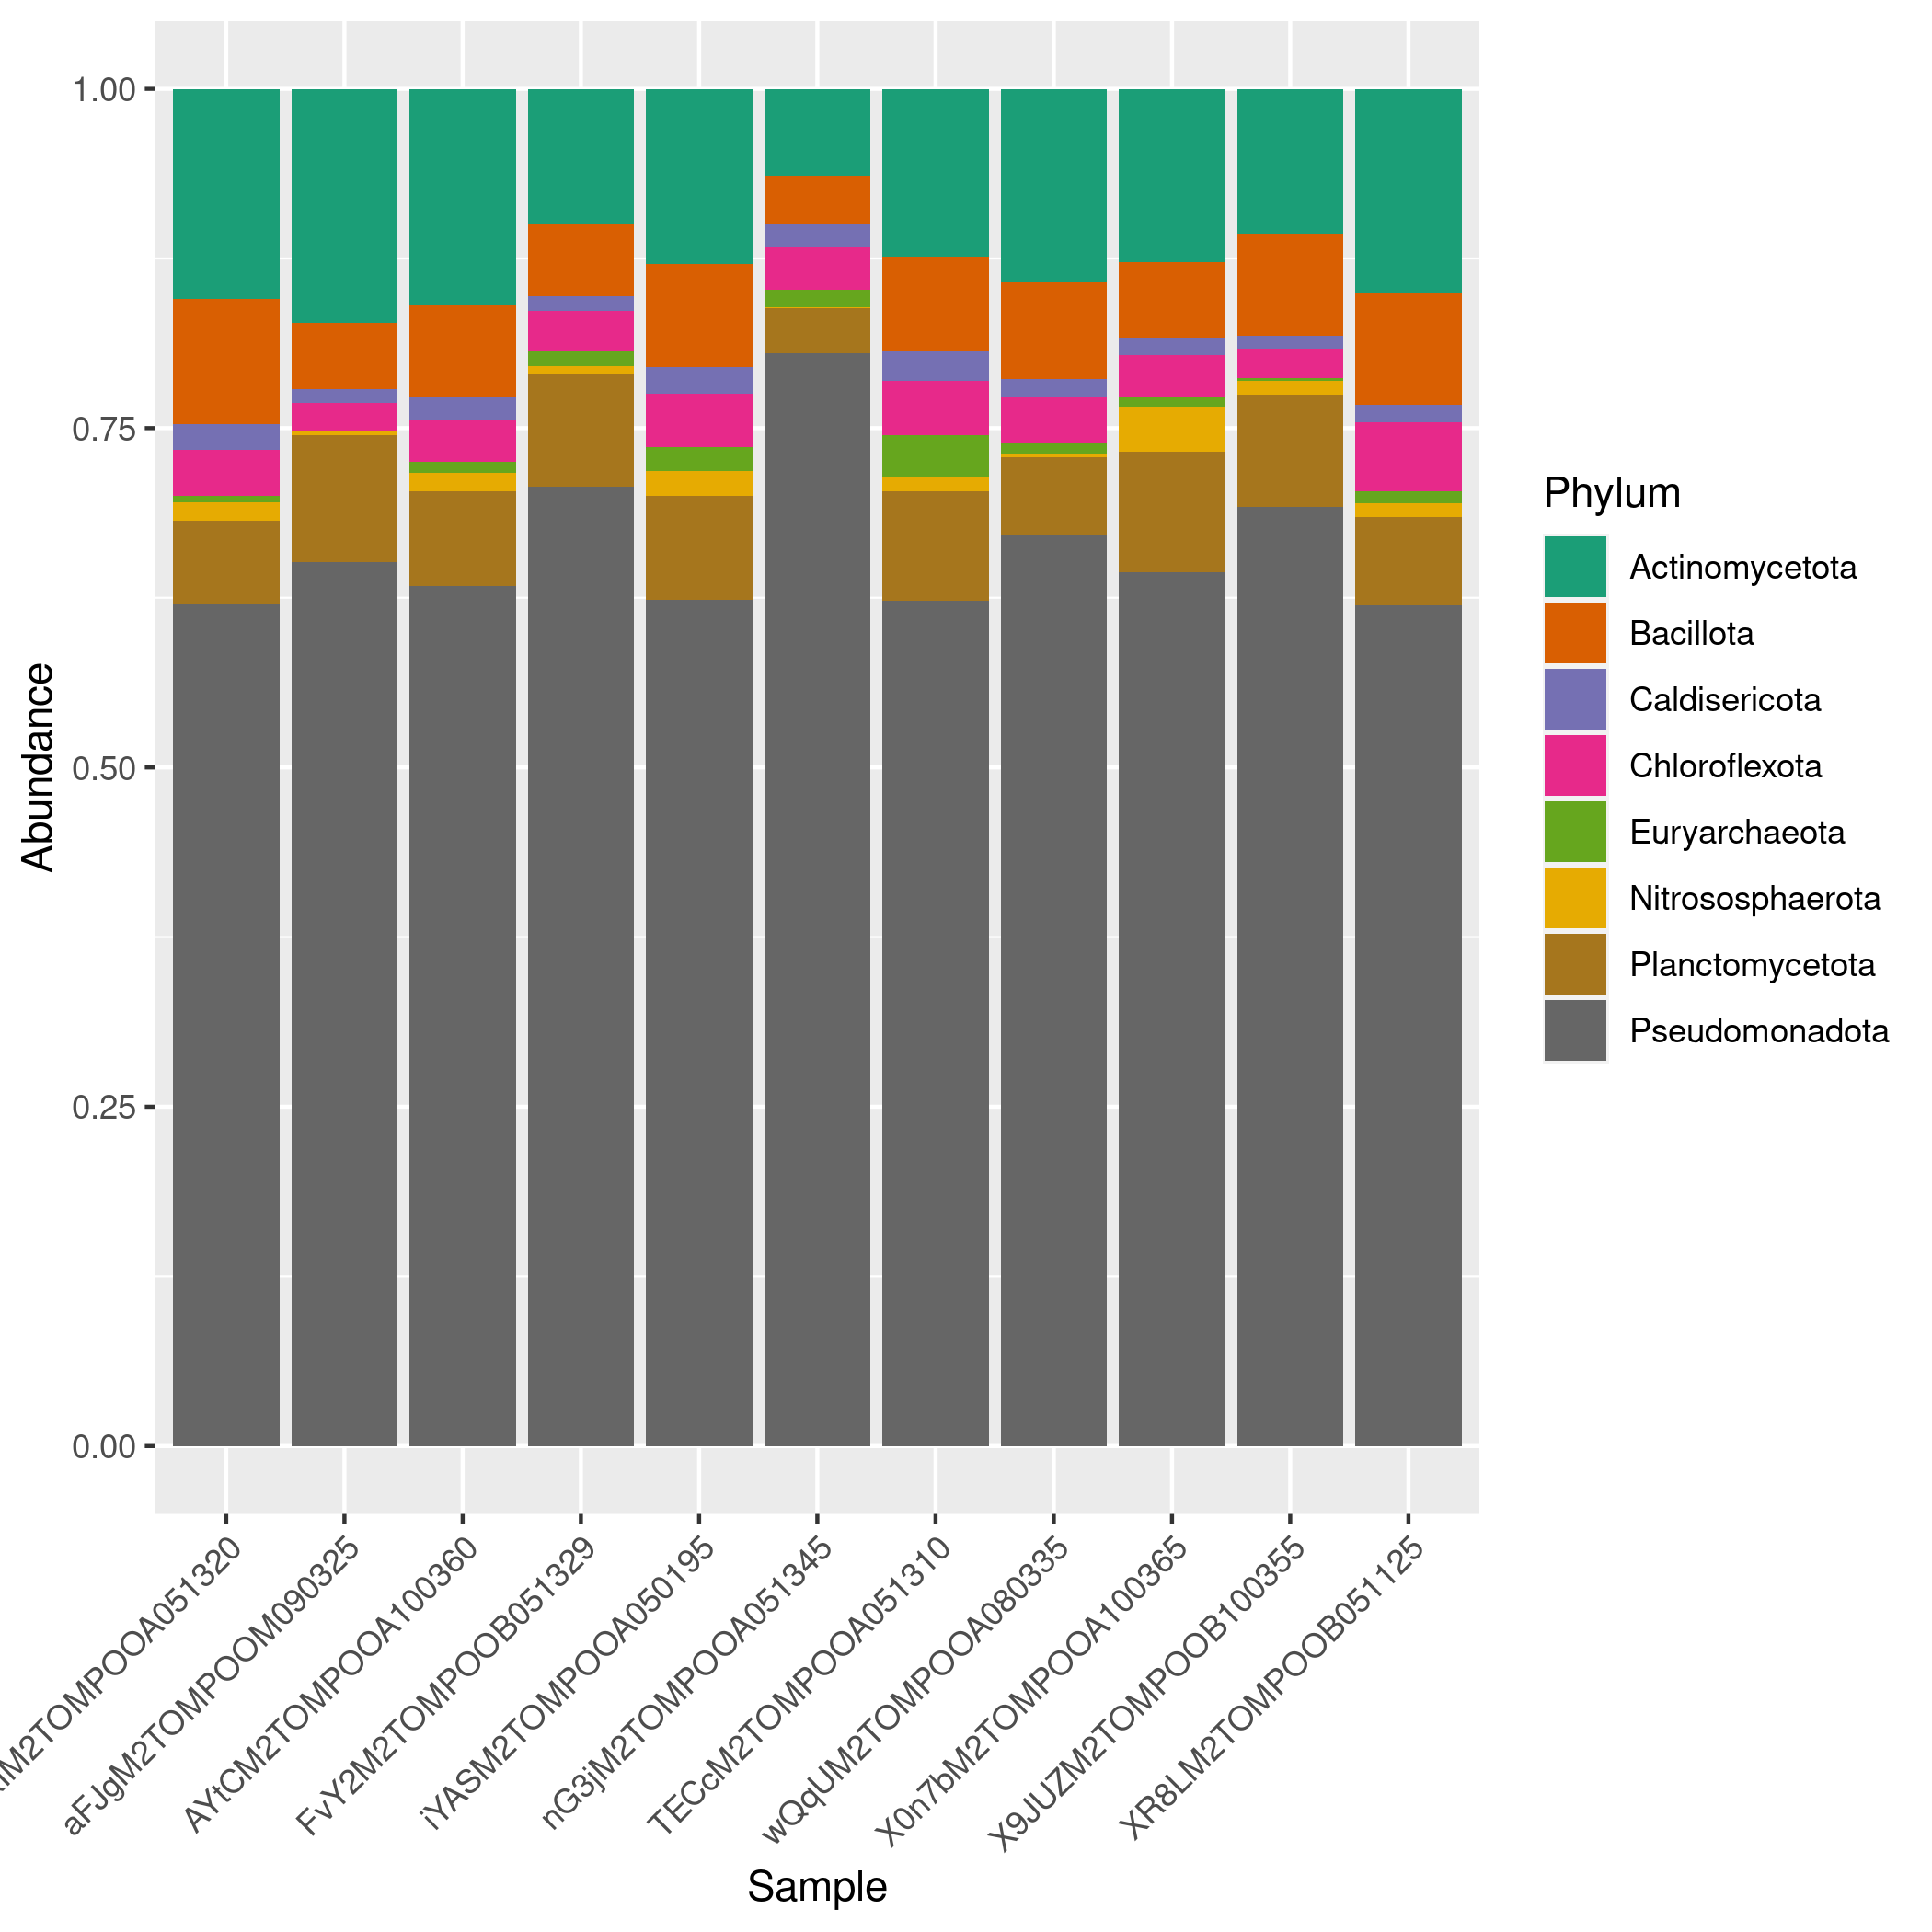
\includegraphics[scale = 0.8]{tomate_aleatorio1_6.csv_relative_abundance_Phylum.png}
\caption{Relative abundance by phyla of keystone OTUs }
\label{fig:tomate_aleatorio1_6.csv_phyla}
\end{figure}
\begin{figure}
\centering
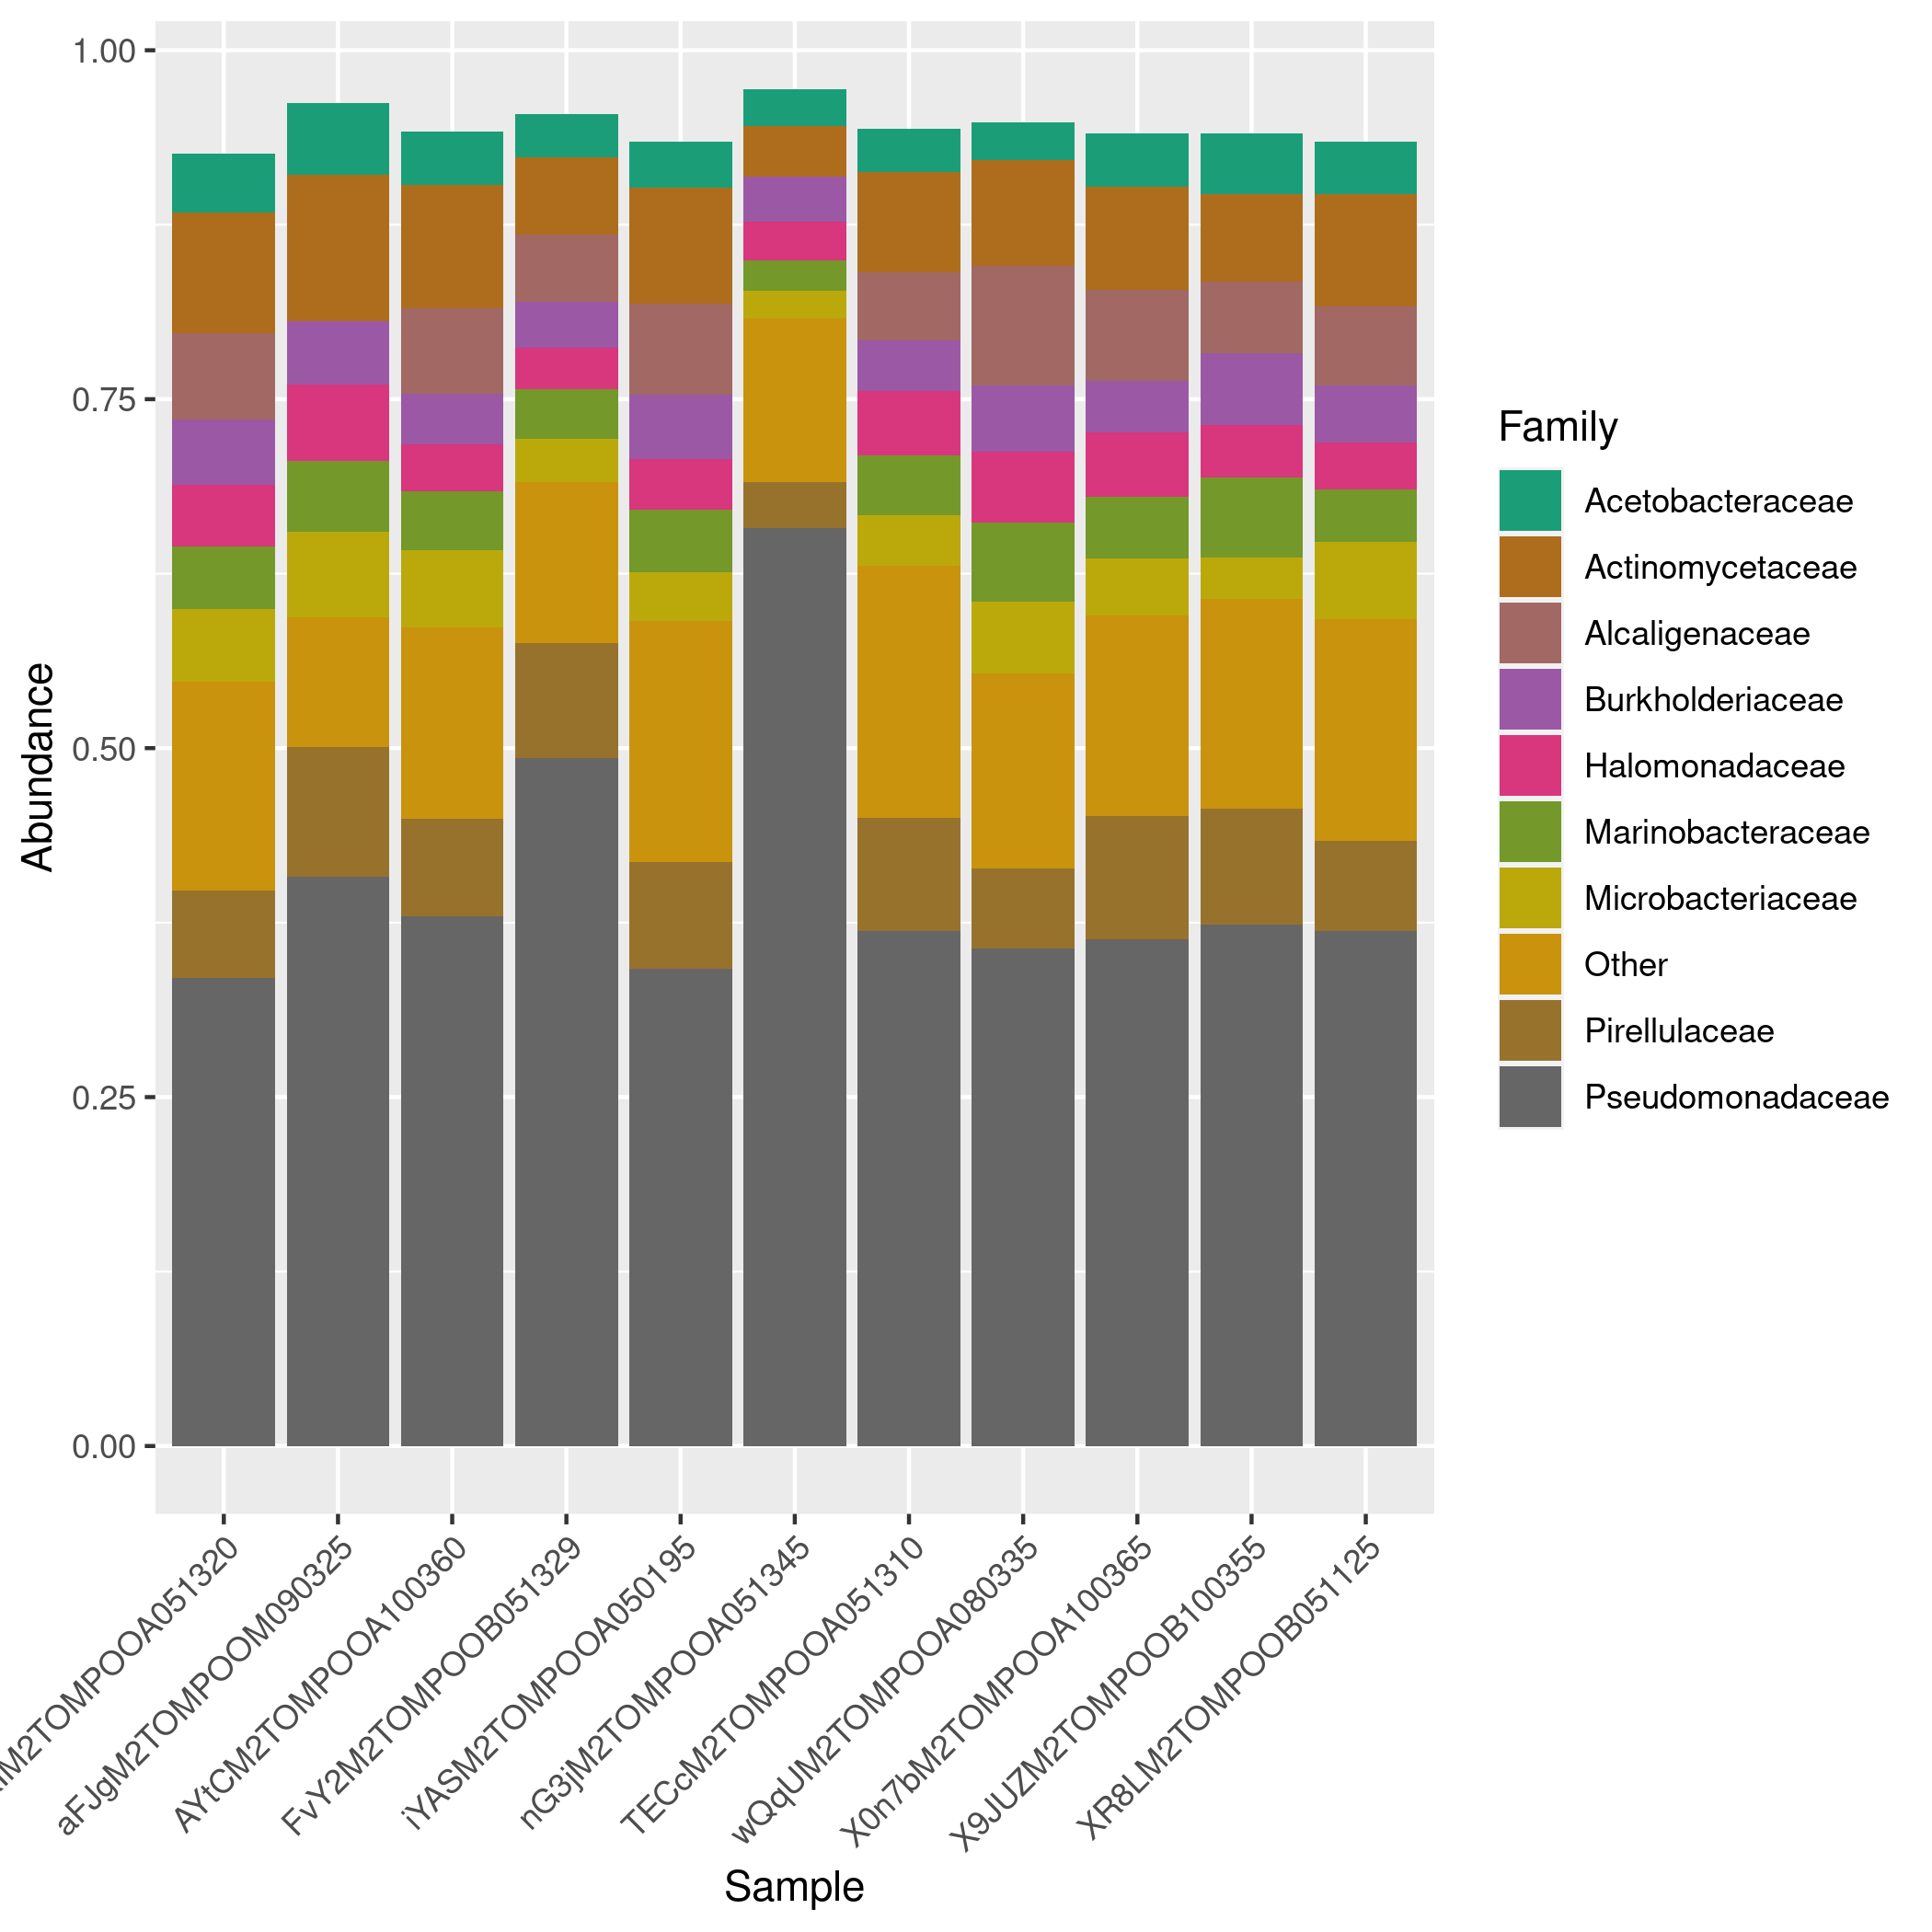
\includegraphics[scale = 0.8]{tomate_aleatorio1_6.csv_relative_abundance_Family.png}
\caption{Relative abundance by families of keystone OTUs }
\label{fig:tomate_aleatorio1_6.csv_family}
\end{figure}
\begin{figure}
\centering
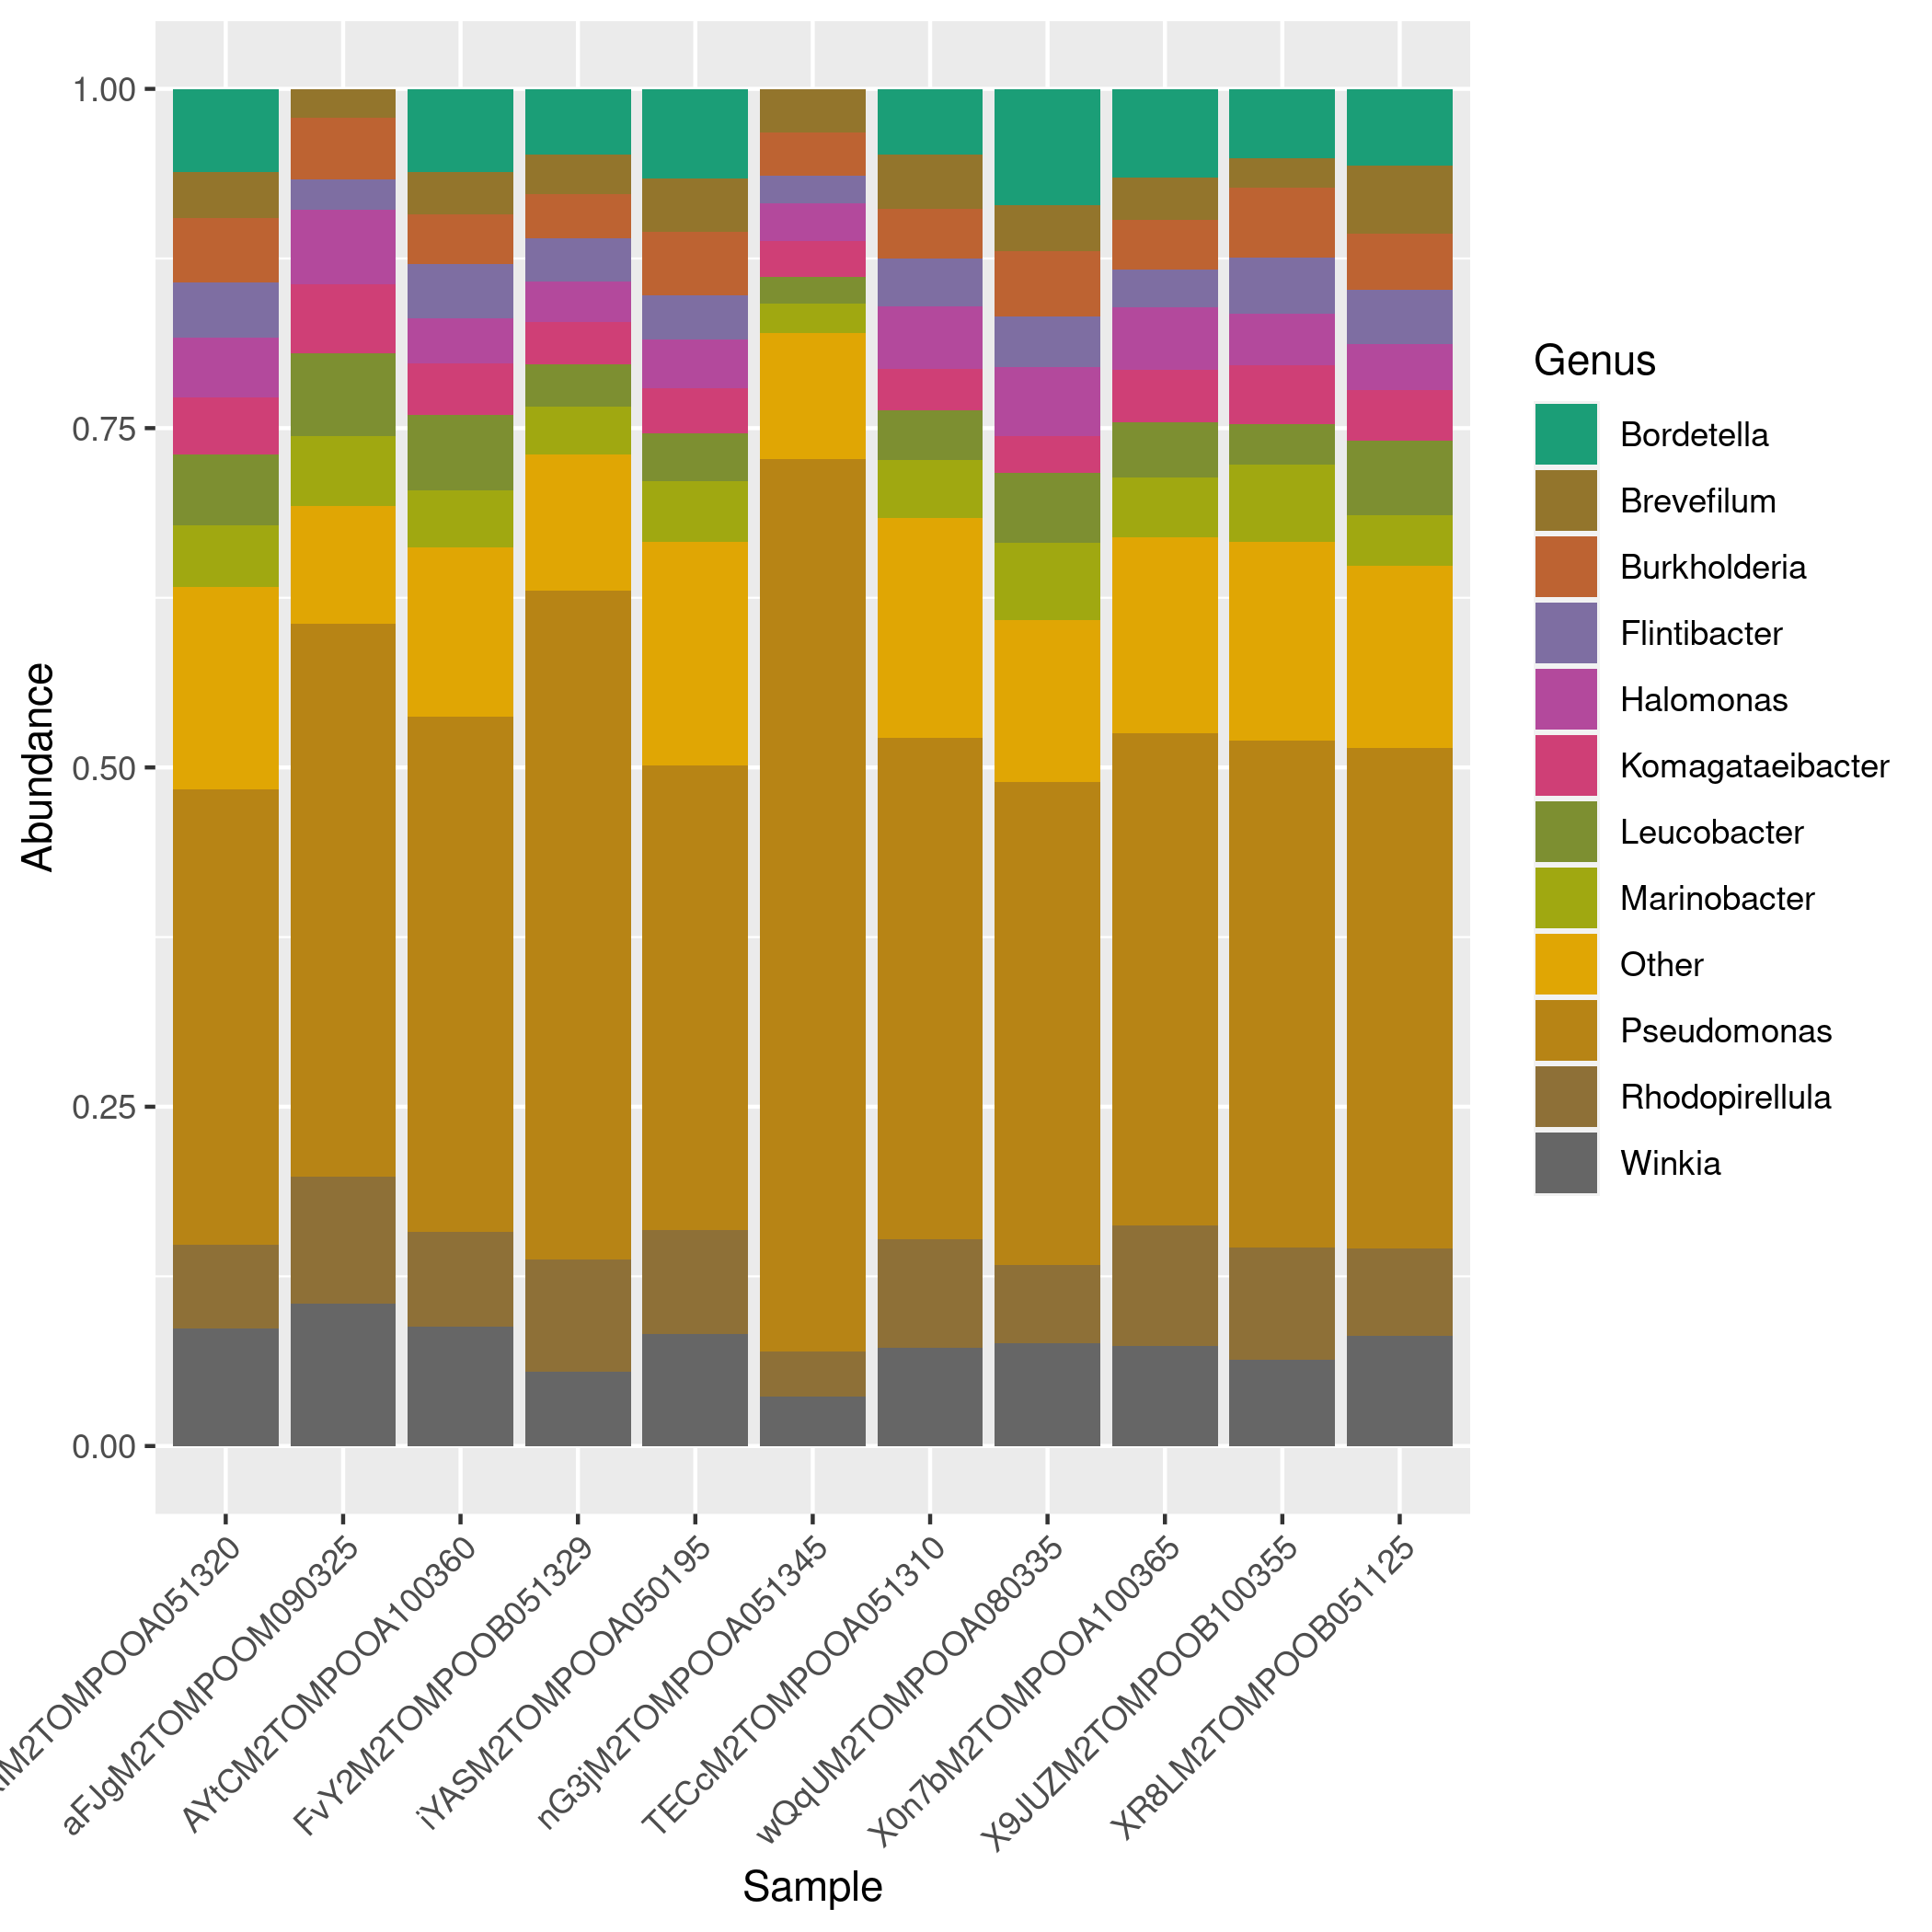
\includegraphics[scale = 0.8]{tomate_aleatorio1_6.csv_relative_abundance_Genus.png}
\caption{Relative abundance by genera of keystone OTUs }
\label{fig:tomate_aleatorio1_6.csv_genus}
\end{figure}
\begin{figure}
   \centering
   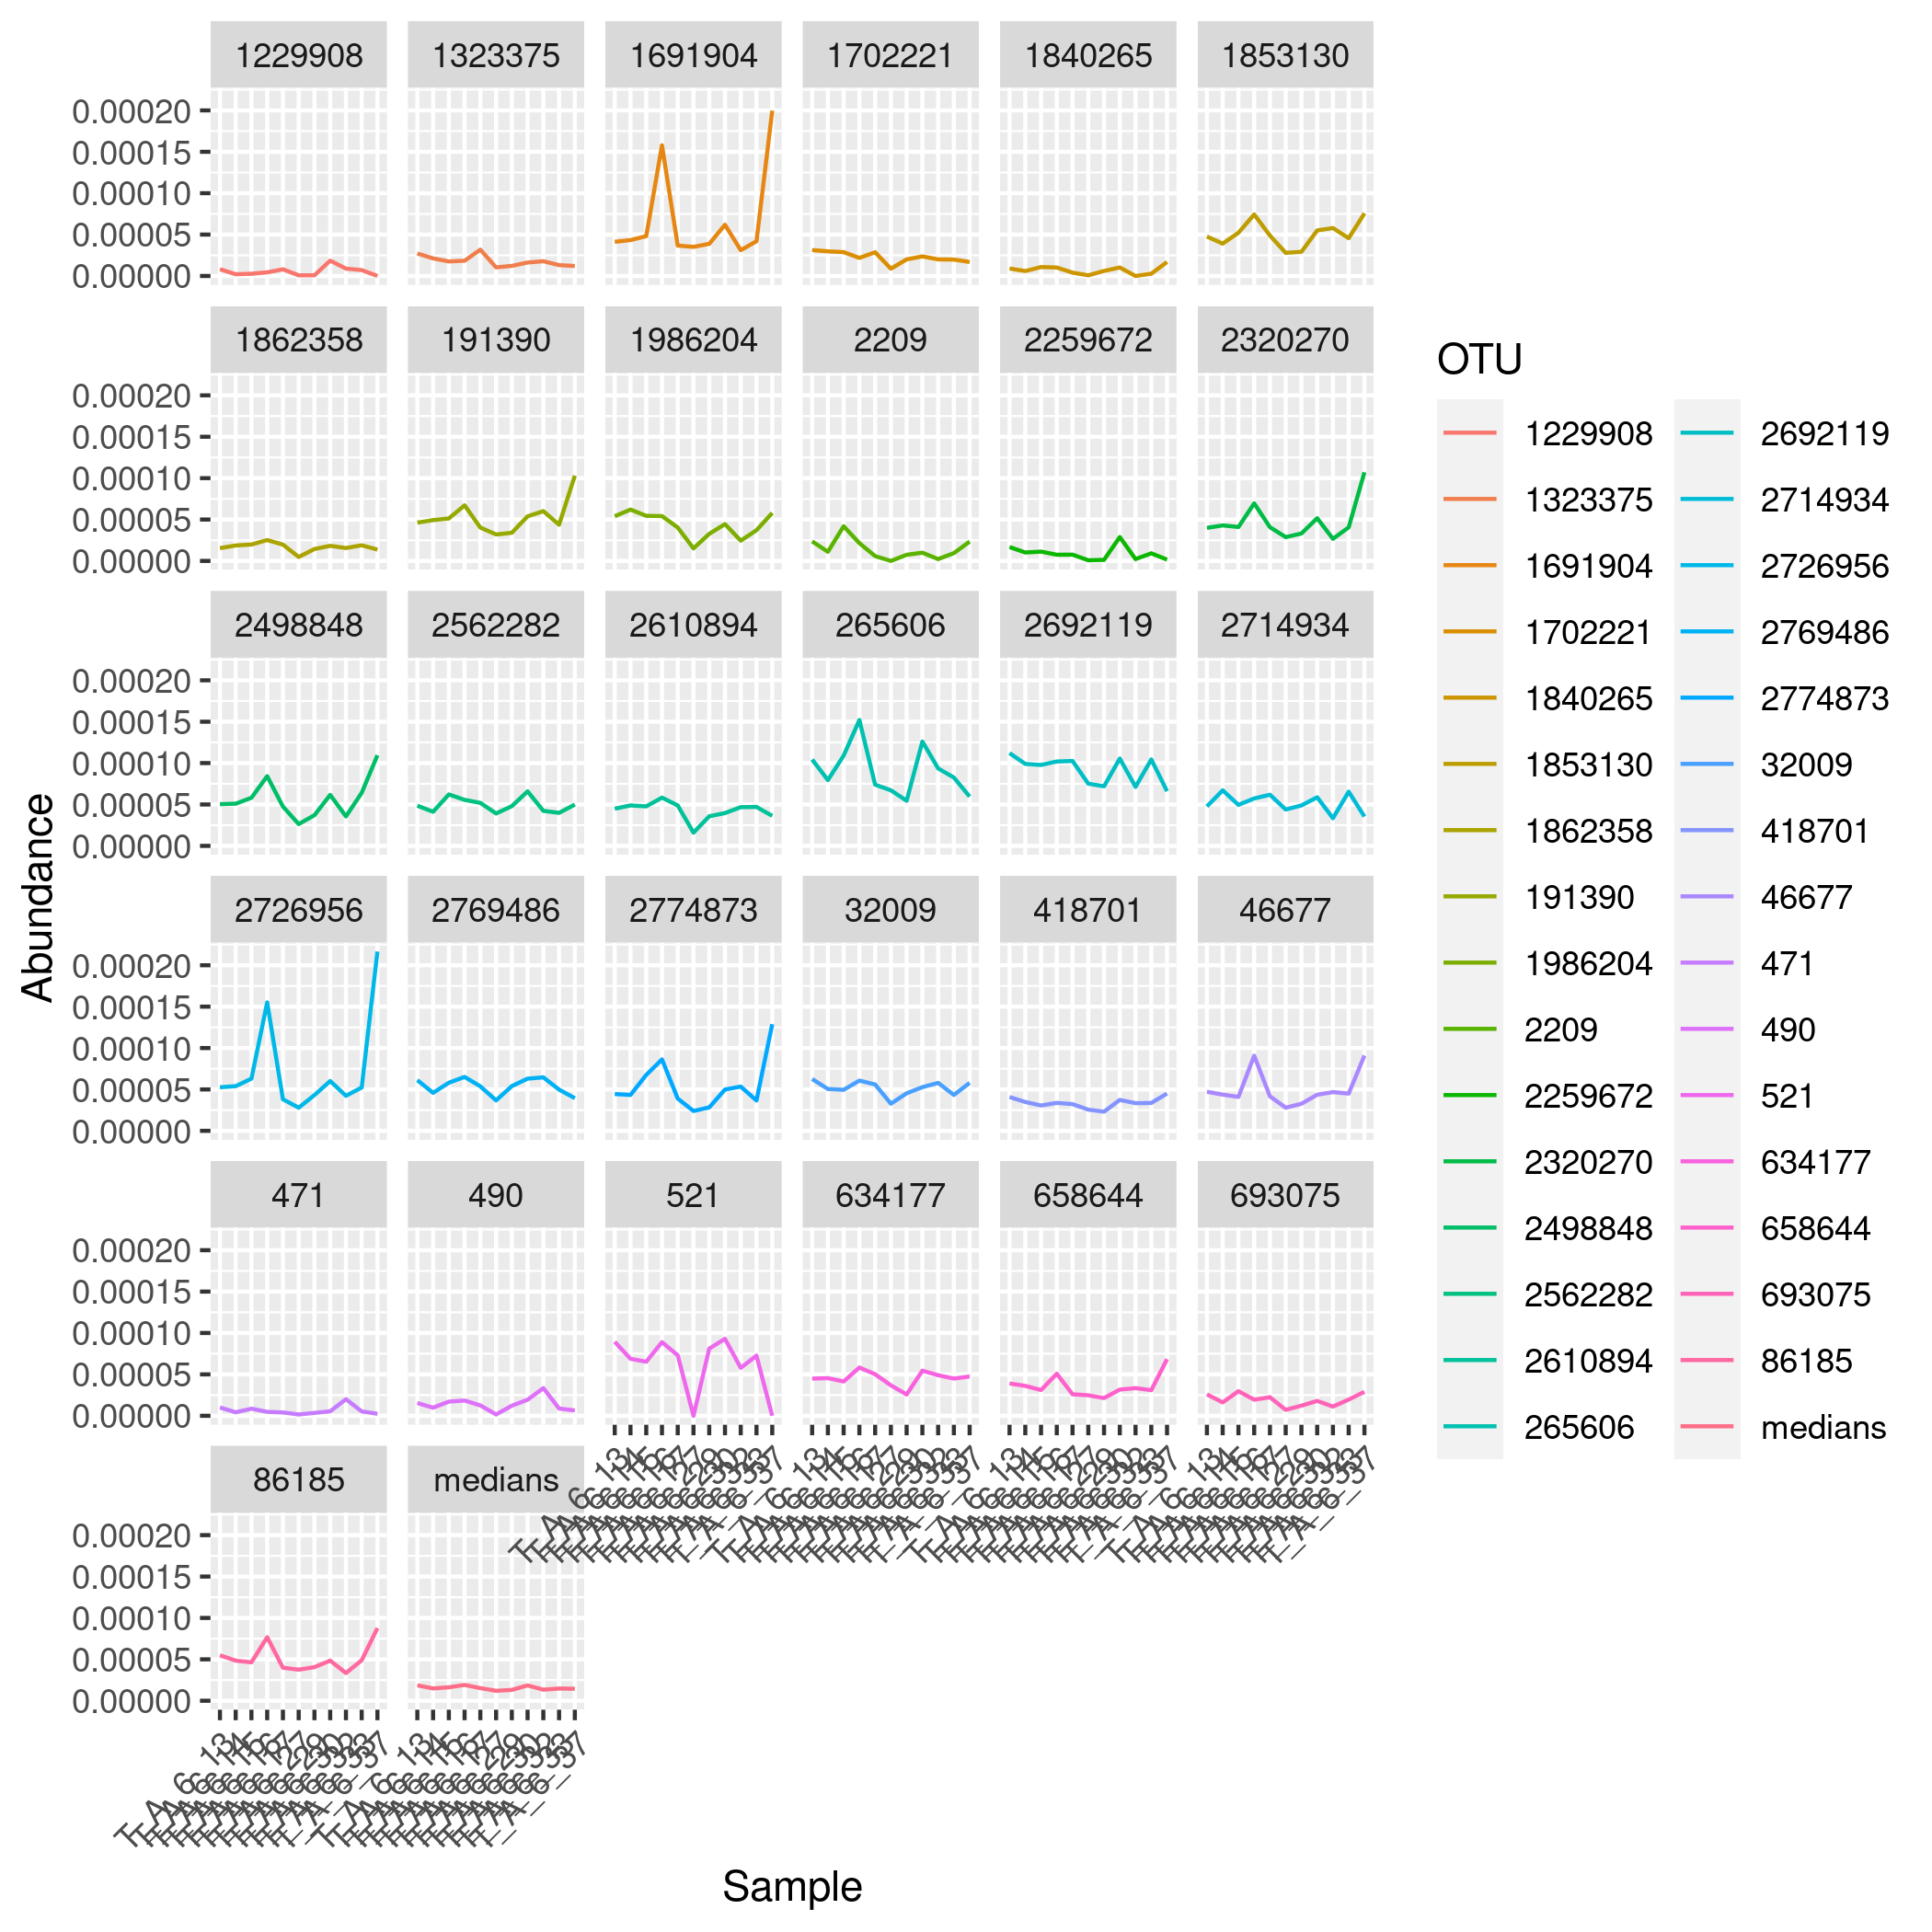
\includegraphics[scale = 0.8]{abundance_tomate_aleatorio1_6.csv_key_otus_medians.png}
   \caption{Plots representing relative abundance of each keystone OTU and one representing the median relative abundance  across samples of rhizosphere of tomate_aleatorio1_6.csv. Most keystone OTUs have relative abundance bigger than the median across all samples.  }
   \label{key_otus_vs_medians_tomate_aleatorio1_6.csv}
\end{figure}
\begin{figure}
 \centering
 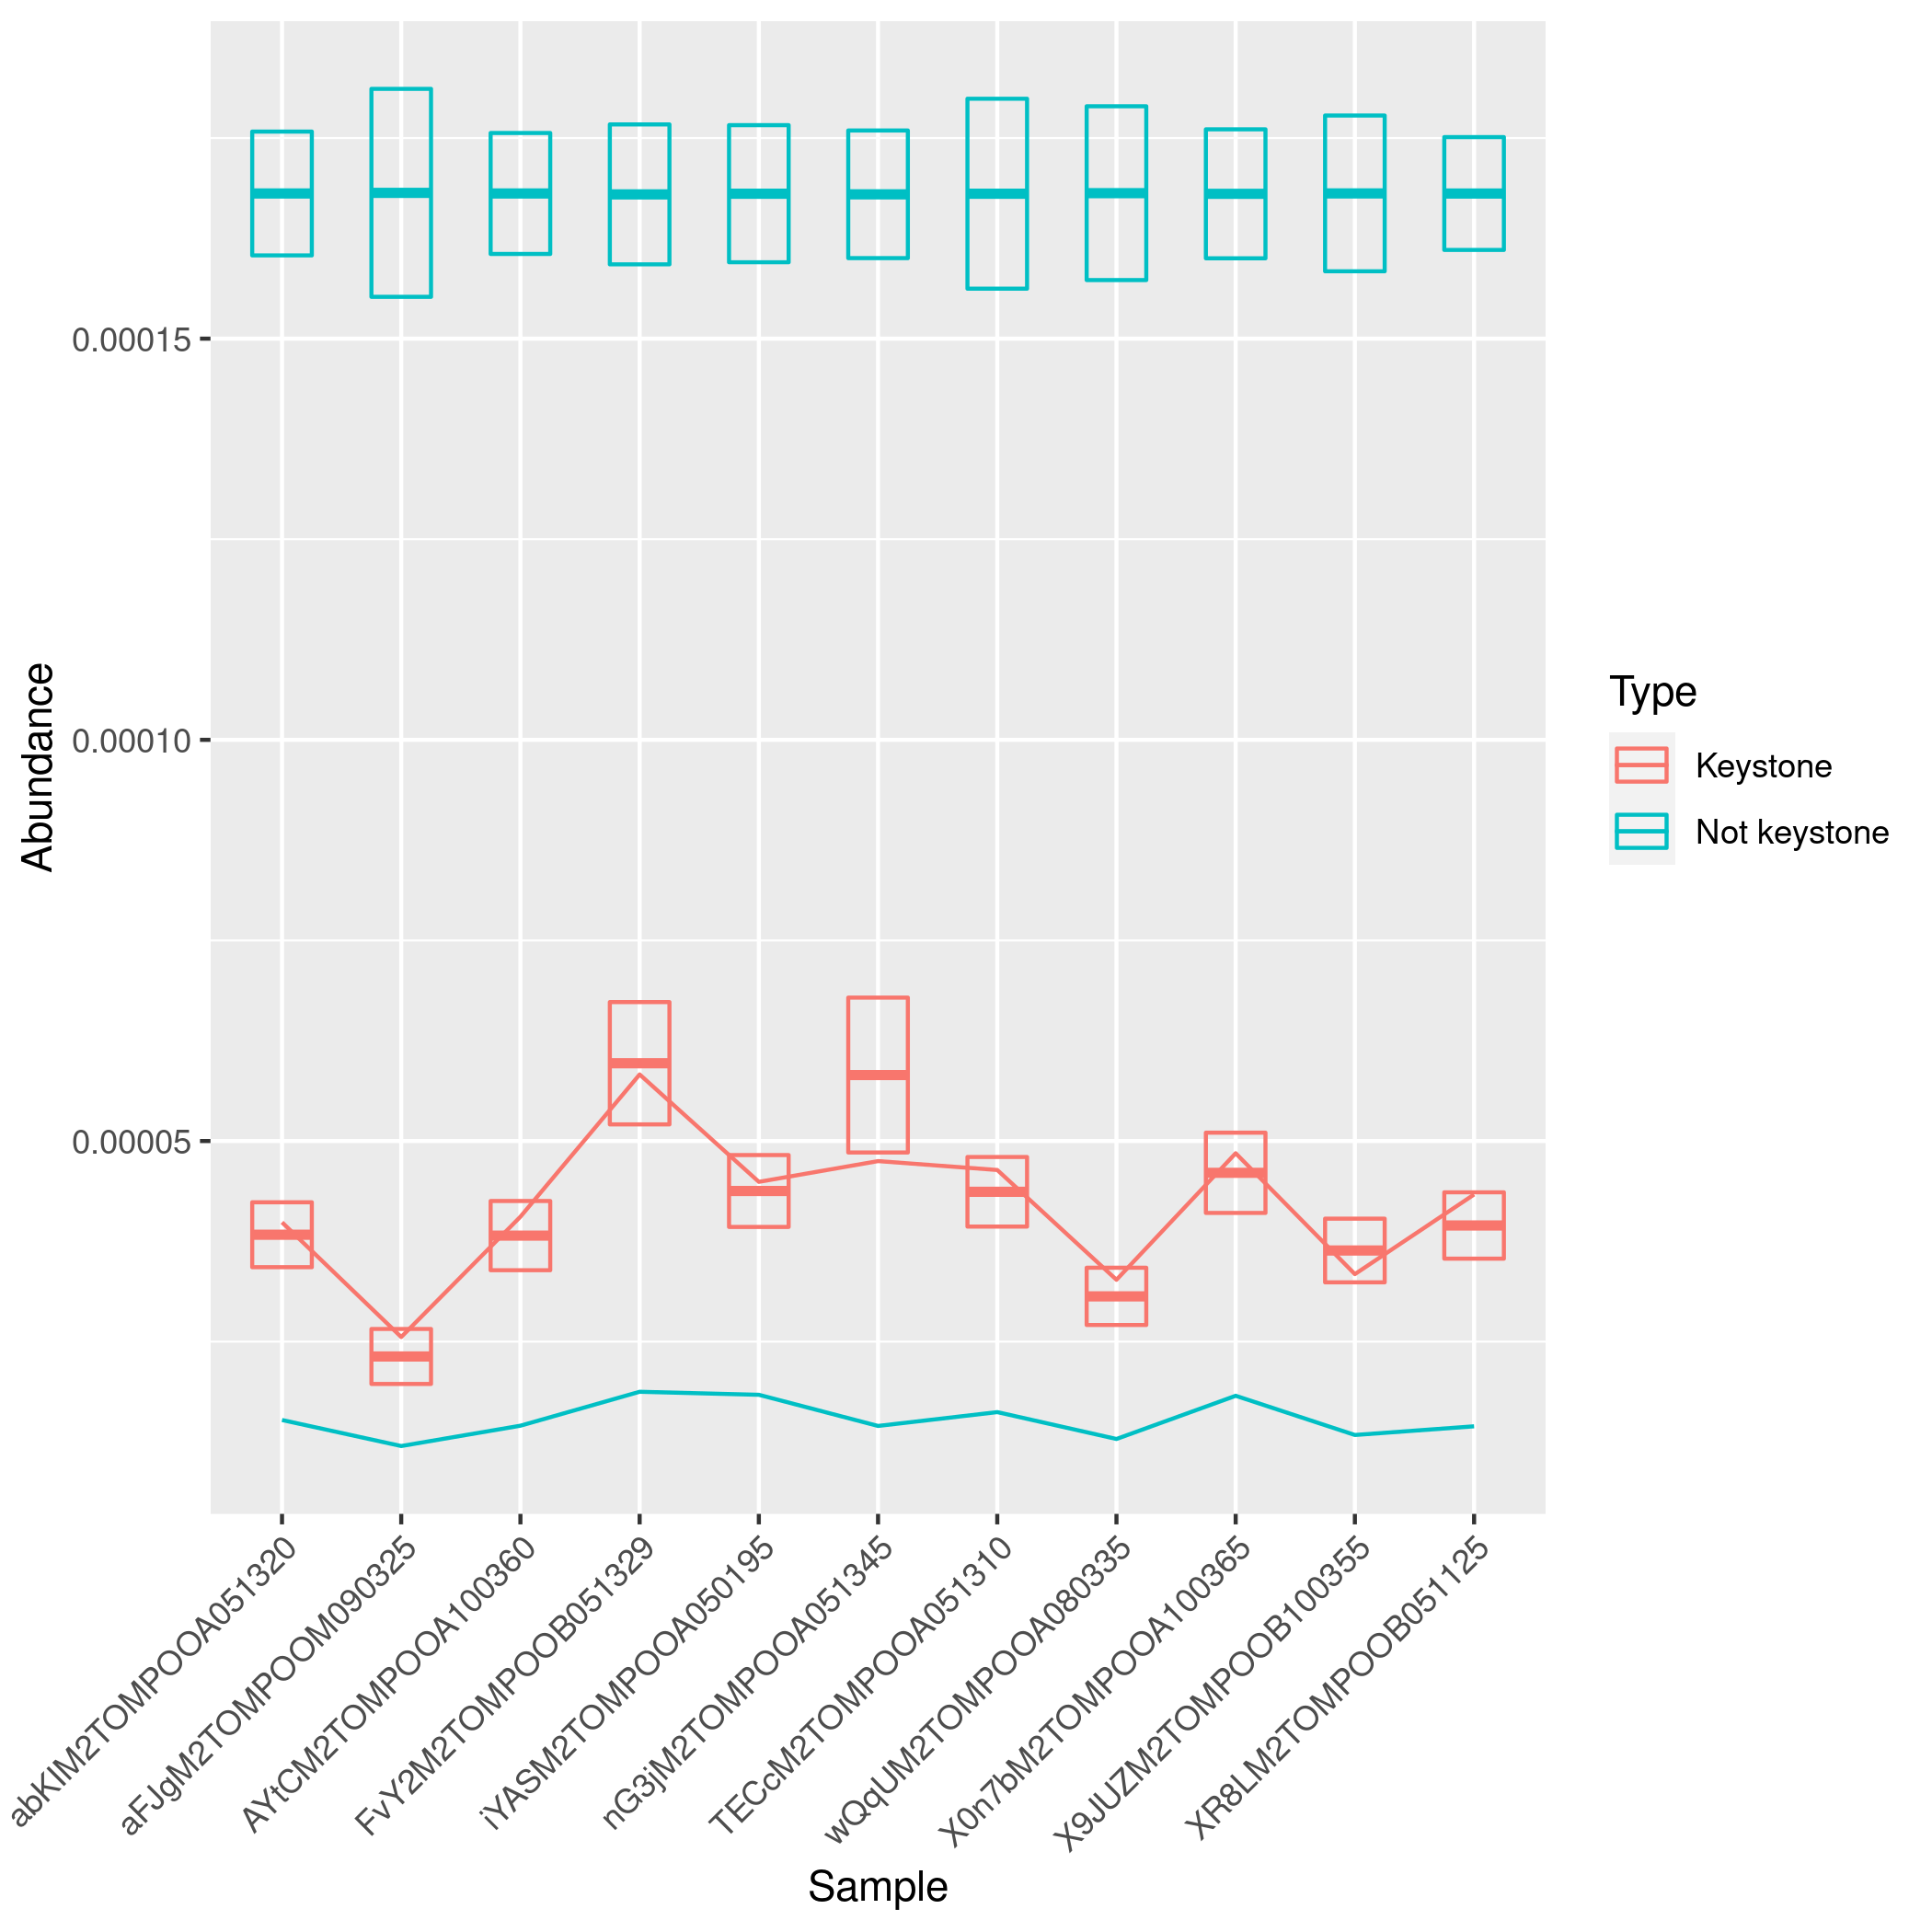
\includegraphics[scale = 0.75]{mean_median_key_vs_not_key_tomate_aleatorio1_6.csv.png}
\caption{Boxes represent mean and standard error in the distribution of corresponding samples. Lines represent the corresponding medians. In these samples of rhizosphere oftomate_aleatorio1_6.csv}
\label{mean_median_tomate_aleatorio1_6.csv}
\end{figure}
\begin{figure}
   \centering
   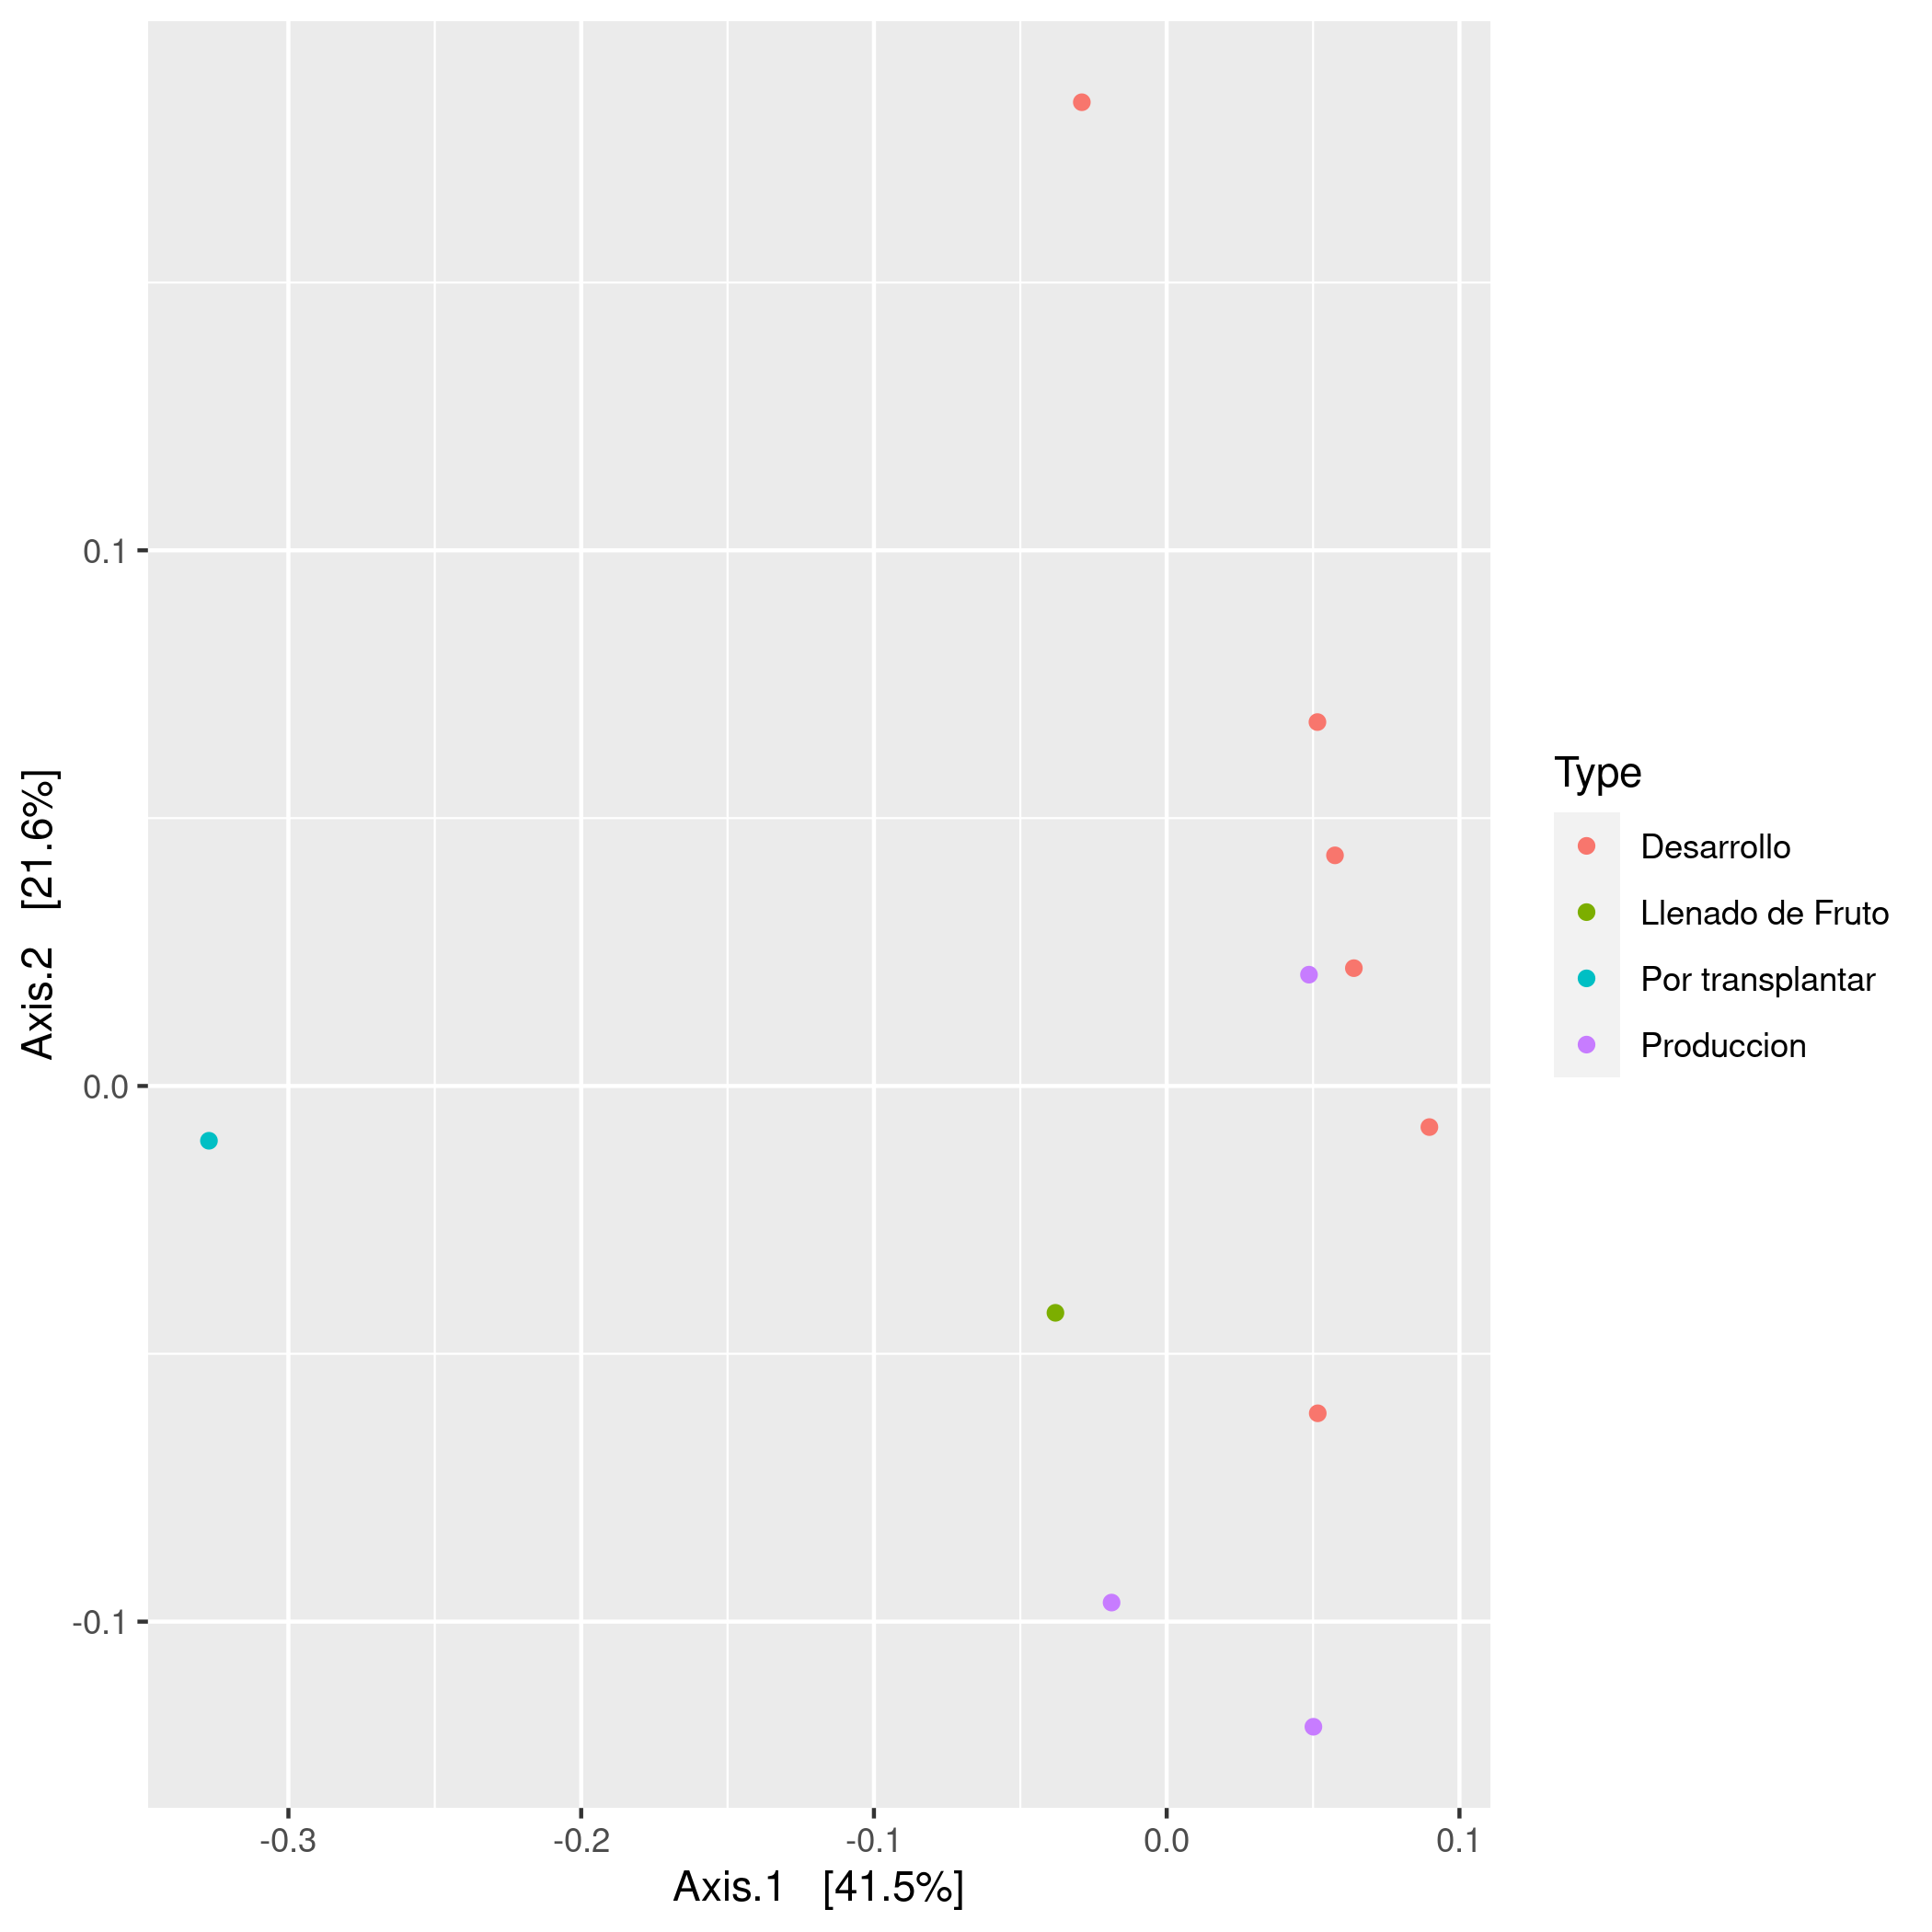
\includegraphics[scale = 0.7]{pcoa_muestras_tomate_aleatorio1_6.csv.png}
 \caption{PCoA analysis with Bray-Curtis distance of rhizosphere samples of tomate_aleatorio1_6.csv.}
 \label{fig:tomate_aleatorio1_6.csv_pcoa}
\end{figure}
\begin{figure}
  \centering
  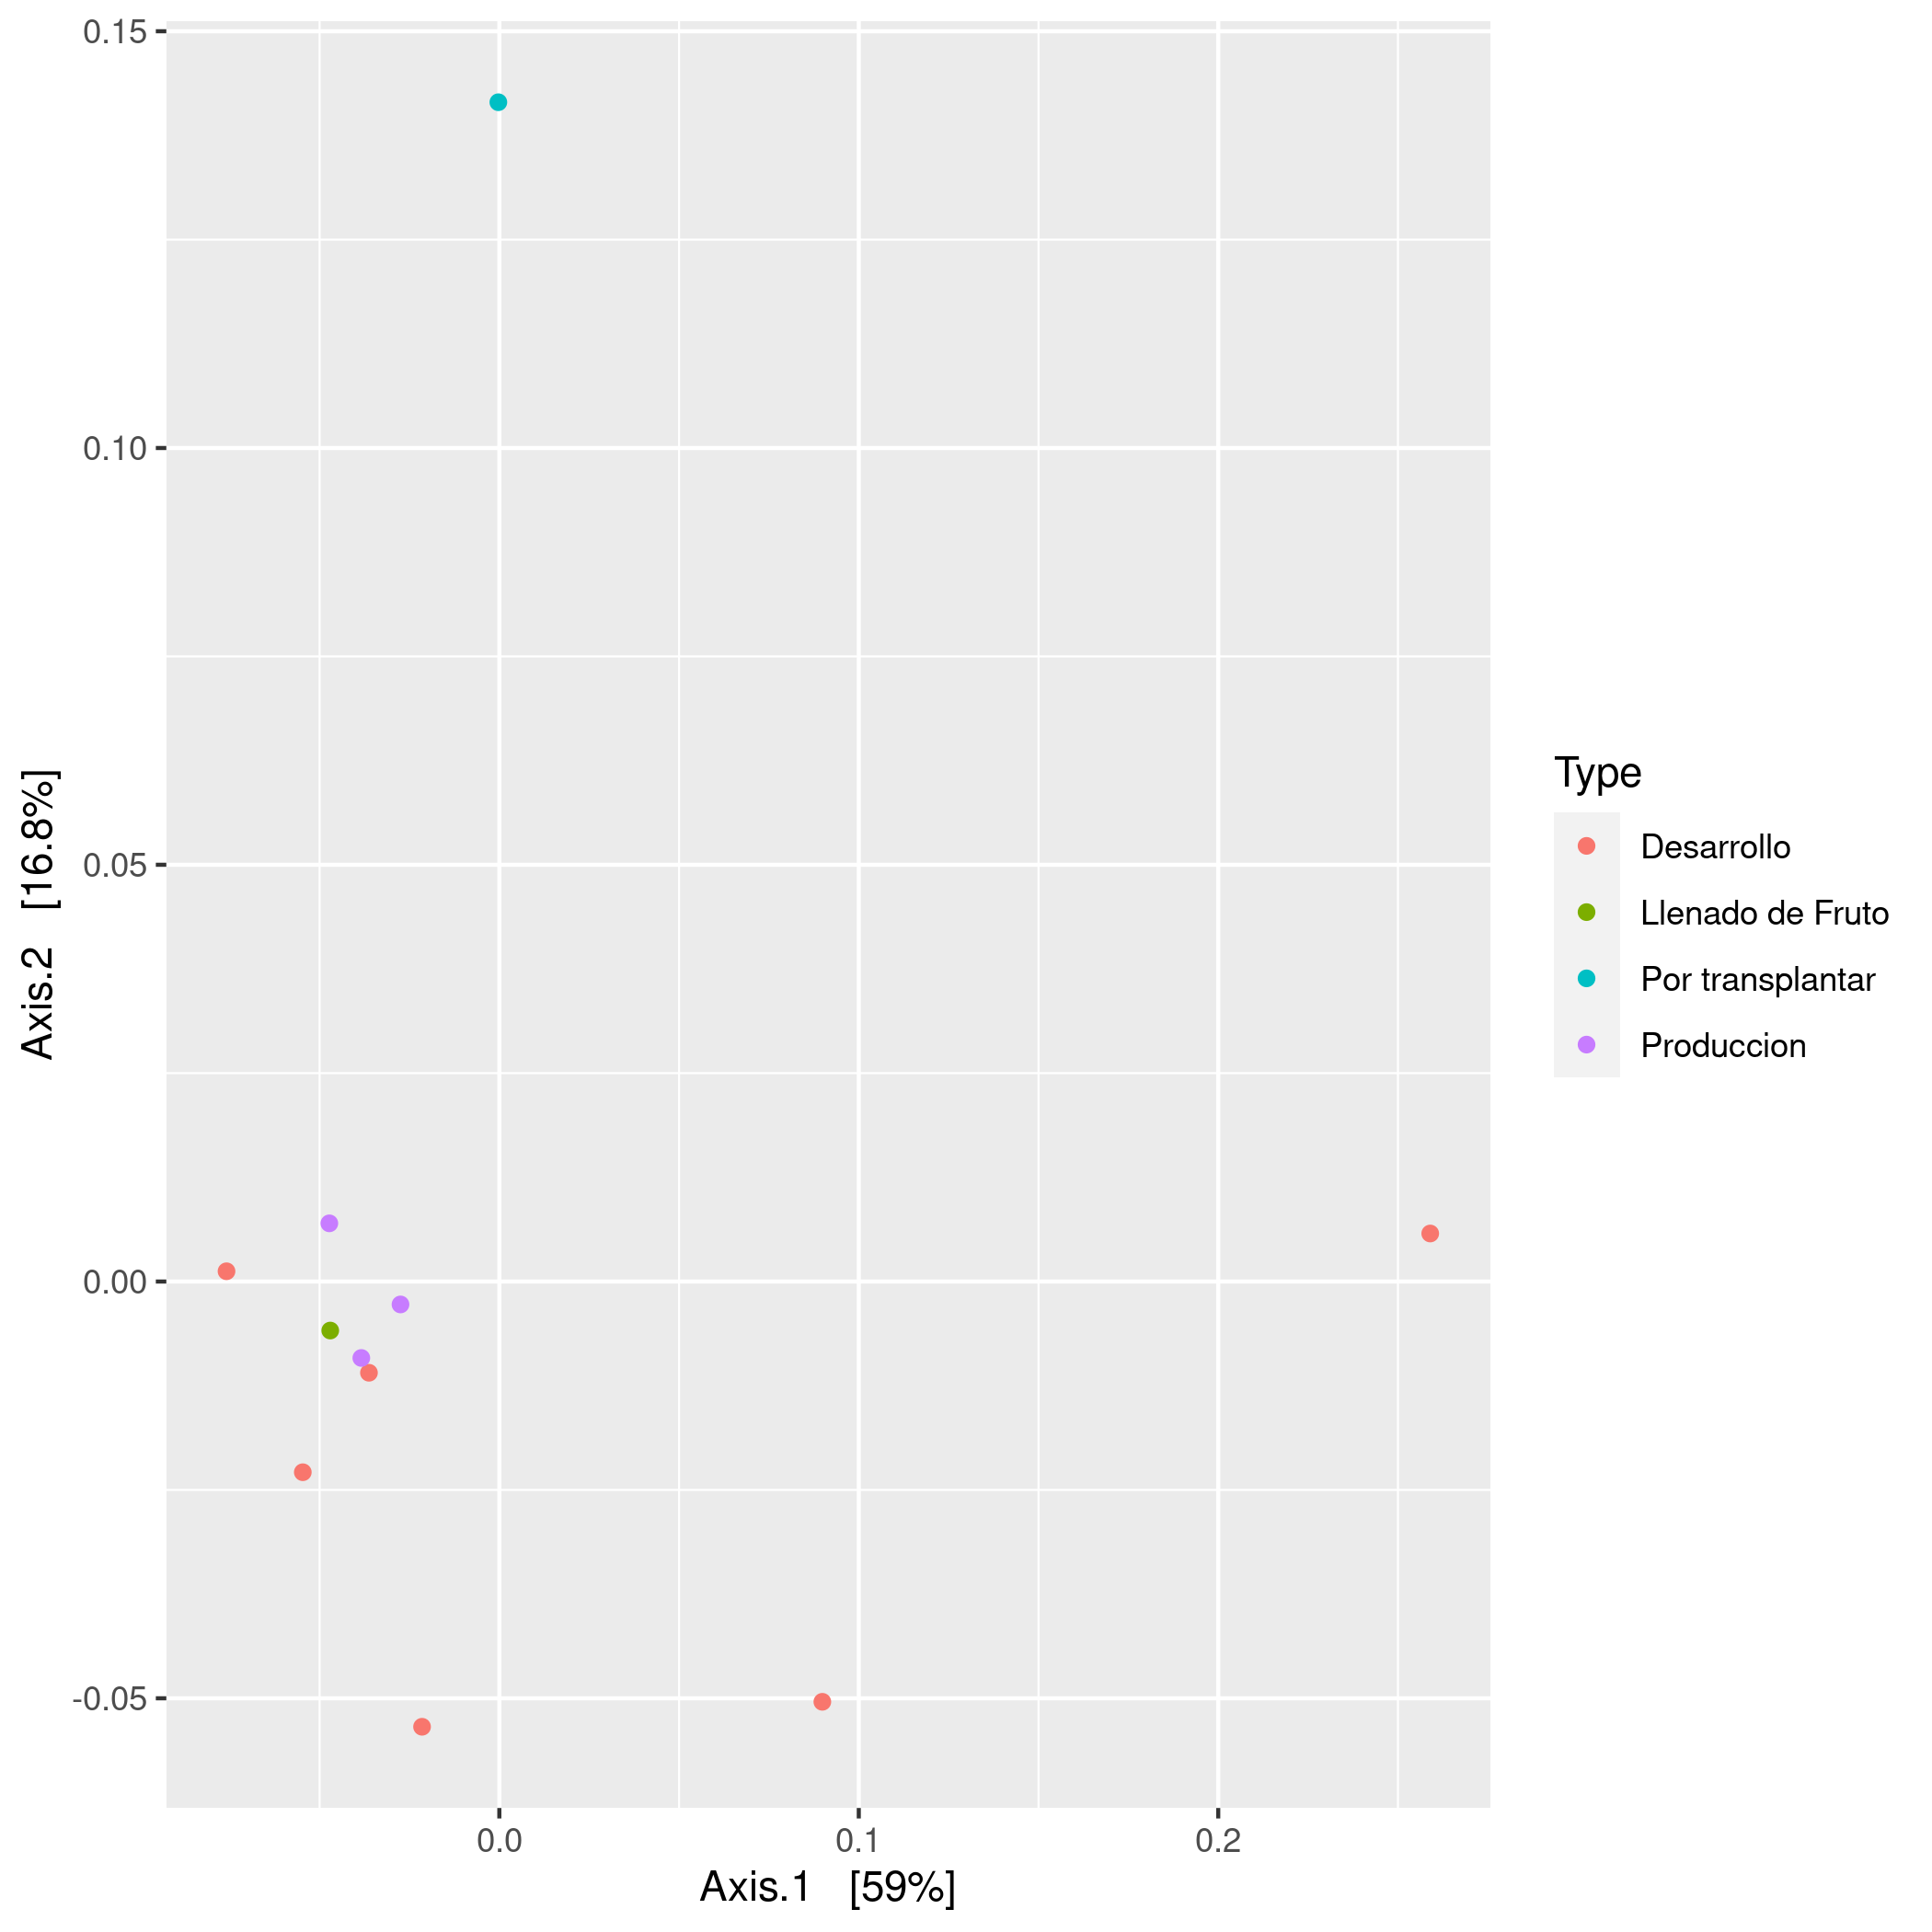
\includegraphics[scale = 0.7]{pcoa_key_otus_tomate_aleatorio1_6.csv.png}
  \caption{PCoA analysis with Bray-Curtis distance of rhizosphere samples of tomate_aleatorio1_6.csv, restricted to keystone OTUs.}
  \label{fig:tomate_aleatorio1_6.csv_pcoa_key_otus}
\end{figure}
